
\section{Functional Requirement}
\begin{table}[h]
\begin{tabular}{|>{\raggedright\arraybackslash}p{5cm}|>{\raggedright\arraybackslash}p{10cm}|}
\hline
\textbf{Functional Requirement}& \textbf{Description }\\
\hline
Login& Allows users to login by their email.\\
\hline
Search product& Finding products on the website with search options such as product name, category, price.\\
\hline
View detail product& Displays detailed information about a product, including product images, description, price, available quantity, and user reviews.\\
\hline
Manage cart& Allows customers to add products to their cart and change the quantity or remove products from the cart before completing their order.\\
\hline
Manage order& Provides order management features for users, including viewing order status, order information, order history, canceling orders, and printing invoices.\\
\hline
Manage inventory and product& Allows repository manager to follow the quantity of products, the history of incoming and outgoing goods, and provided detailed information about each product such as remaining quantity, quantity sold, etc.\\
\hline
Manage promotion & Allow admin and sales employee create and manage promotion, and provide for customer.\\
\hline
Manage post & Marketing employee can create, delete, edit post/blog. \\
\hline
Order & Enables the system to process orders and notify customers about the status of their order, delivery time.\\
\hline
Send support request & Customer can send request to customer care employee.\\
\hline
Statistics& Provides reporting and analytics features for admin to evaluate the website's business performance, such as revenue, top-selling products, and other metrics.\\
\hline
\end{tabular}
\caption{Functional Requirement}
\label{tab:Functional }
\end{table}
\section{Non-functional Requirement}
\begin{table}[H]
\begin{tabular}{|>{\raggedright\arraybackslash}p{5cm}|>{\raggedright\arraybackslash}p{10cm}|}
\hline
\textbf{Non-Functional Requirement} & \textbf{Description} \\
\hline
Compatibility and universality& Login Operate on different devices and browsers.\\
\hline
Quick responsiveness&The website has a fast page load speed to ensure a good user experience.\\
\hline
High security &Protect the personal information of customers and transactions.\\
\hline
User-friendly  interface& Easy to use and suitable for users.\\
\hline
 Scalability& Able to expand.\\
\hline
Product reliability&Users will evaluate the product and can view the reviews of other users before deciding to make a purchase.\\
\hline
\end{tabular}
\caption{Non-Functional Requirement}
\label{tab:Non-Functional}
\end{table}


\section{Functional Diagram of System}
\subsection{Use-Case Diagram}

\begin{figure}[H]
  \centering
  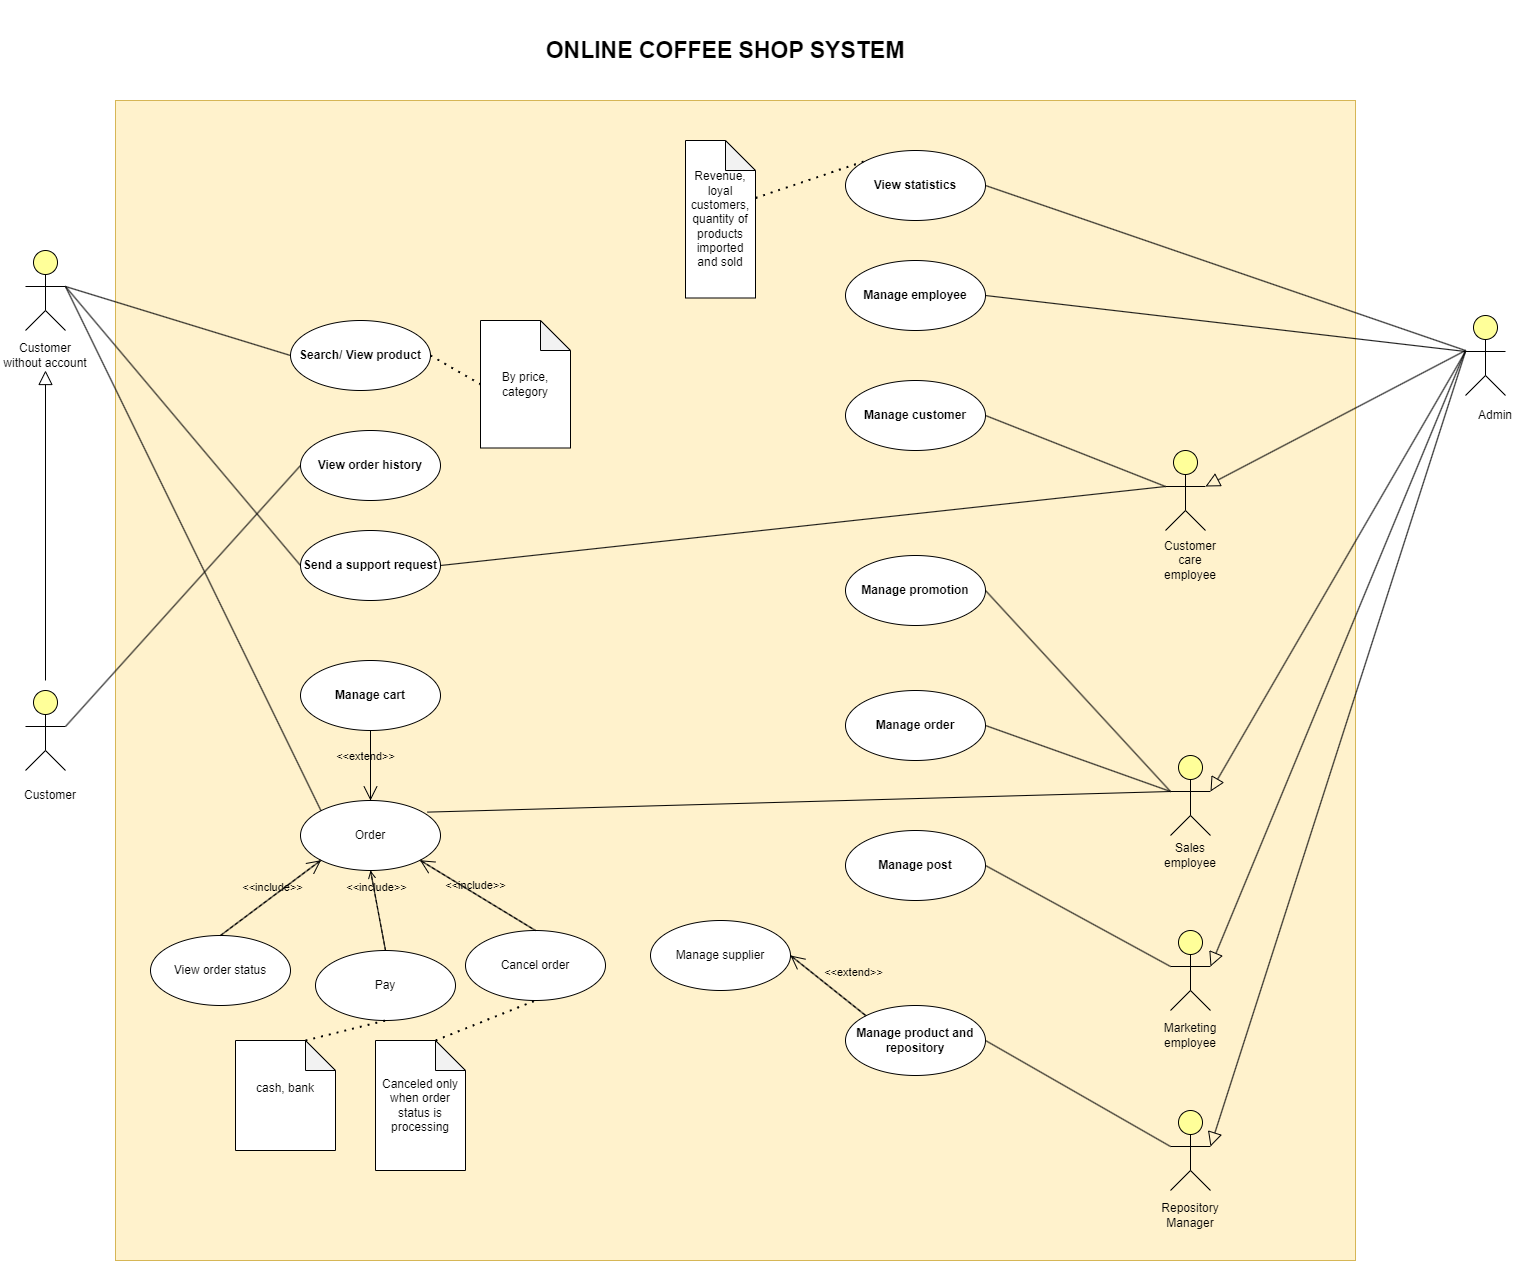
\includegraphics[width=1.1\textwidth]{UseCase.png}
  \caption{Use-case Diagram}
  \label{fig:usecase}
\end{figure}
%Use-case tổng quát và chi tiết
\subsection{Use-Case Description}
% Số lượng actors, usecases
There are 7 actors and 13 Use-cases.

\begin{table}
\begin{tabular}{|>{\raggedright\arraybackslash}p{6cm}|>{\raggedright\arraybackslash}p{10cm}|}
\hline
\textbf{Actors}& \textbf{Description}\\
\hline
\multirow{2}{*}{Customer without an account}& Search/View product \\
& Manage cart\\
& Send a support request\\
\hline
\multirow{2}{*}{Customer}& View order history \\
& Customer without account's rights. \\
\hline
\multirow{2}{*}{Sales employee}& Manage promotion \\
& Manage order\\
\hline
Customer care employee& Manage customer's information\\
\hline
Repository manager& Manage product and repository\\
\hline
Marketing employee& Manage post\\
\hline
\multirow{3}{*}{Admin}& View statistics\\
& Manage employee \\
& All right of employees\\
\hline
\end{tabular}
\caption{List of actors of system}
\label{tab:actors}
\end{table}

%list of use-cases
\begin{table}
\begin{tabular}{|>{\raggedright\arraybackslash}p{1cm}|>{\raggedright\arraybackslash}p{3cm}|>{\raggedright\arraybackslash}p{8cm}|>{\raggedright\arraybackslash}p{3cm}|}
\hline
\textbf{ID}& \textbf{Use-Case}& \textbf{Description}& \textbf{Actor}\\
\hline
UC01& Login& Actor login to the system. Depending on the account type, there are different functions& Admin, Customer, Employees \\
\hline
UC02& View statistics& View sales statistics, purchase rate of products, potential customers& Admin\\
\hline
UC03& Manage employee& It is a tool to manage admin account, divide role.
View, create, lock, unlock accounts& Admin\\
\hline
UC04& Manage customer& Actor manages customer information by viewing, deleting, and editing customer information and actions& Admin, Customer care employee\\
\hline
UC05& Manage product and repository& Manage products by add, edit or delete. Import products from suppliers& Admin, Repository manager\\
\hline
UC06& Manage post& Actor manages the content of articles about the store, privacy policy and terms of use, articles promoting the company& Admin, Marketing employee\\
\hline 
UC07& Manage promotion& Actor adjusts promotions, promotions of each product, product according to the manufacturer& Sales employee\\
\hline
UC08& Manage order& Actor reviews orders, approves orders, transfers them to shipping department& Admin, Sales employee\\
\hline
UC09& Send a support request& In the process of using the software, if there is an error, the actor sends a support request for the system employee to handle& Admin, Customer care employee, Customer\\
\hline
UC10& Search/View product& User can view, search, and filter products of the shop& Customer\\
\hline
UC11& Manage cart& User can create cart, add product to cart, control the
amount of product& Customer \\
\hline
UC12& Order& User can complete their order, see all stuff, edit address,
choose the payment method. If users choose online
payment, they can buy it automatically& Customer\\
\hline 
UC13& View order history& User can see their history of buying products from the
services& Customer\\
\hline 
\end{tabular}
\caption{List of Use-Cases of system}
\label{tab:use-cases}
\end{table}




% đặc tả
%mỗi bảng đặc tả bao gồm tên Use-case, tác nhân chính và phụ, mô tả, hoạt động/ tác nhân kích hoạt, mối quan hệ Use-case (Include/Extend), luồng hoạt động chính, luồng hoạt động thay thế
% UC01
\begin{table}
\begin{tabular}{|>{\raggedright\arraybackslash}p{5cm}|>{\raggedright\arraybackslash}p{10cm}|}
\hline
ID& UC01 \\
\hline
Use-Case Name& Login\\
\hline
Actors& Customer, Admin and employees\\
\hline
Primary Actors& Customer, Admin and employees\\
\hline
Brief Description& Login is the process of verifying a user's identity and granting access to system, application, website. It involves authentication OAUTH2.\\
\hline
Trigger& User click the Login button\\
\hline
Relationships& \\
\hline
Flow& The user clicks on the "Sign in with Google" button, which redirects them to the Google OAUTH authorization server.
The user is prompted to enter their Google credentials and to grant permission to the system to access their Google account information.
If the user grants permission, the Google OAuth authorization server sends a token to the system that proves the user has been authenticated.
The system uses this token to retrieve the user's Google account information from Google's servers, such as their name, email address, and profile picture.\\
\hline
Subflows&\\
\hline
\end{tabular}

\caption{UC01 Login}
\label{tab:UC01}
\end{table}
% UC02
\begin{table}
\begin{tabular}{|>{\raggedright\arraybackslash}p{5cm}|>{\raggedright\arraybackslash}p{10cm}|}
\hline
ID& UC02\\
\hline
Use-Case Name& View statistics\\
\hline
Actors& Admin\\
\hline
Primary Actors& Admin \\
\hline
Brief Description& It is a mathematical tool used to analyze and interpret data. It is used to summarize data by time given. It can also be used to make predictions about future data for improving the business. The function give overview about income, which product has most people buy, receipt by status\\
\hline
Trigger& Admin click the Statistic menu\\
\hline
Pre-conditions& User must login first \\
\hline
Relationships& \\
\hline
Flow& Choose things to statistic: Revenue, product\\
\hline
Subflows& \\
\hline
\end{tabular}
\caption{UC02 View Statistics}
\label{tab:UC02}
\end{table}
% UC03
\begin{table}
\begin{tabular}{|>{\raggedright\arraybackslash}p{5cm}|>{\raggedright\arraybackslash}p{10cm}|}
\hline
ID& UC03 \\
\hline
Use-Case Name& Manage employee\\
\hline
Actors& Admin, employee\\
\hline
Primary Actors& Admin\\
\hline
Brief Description& It is a tool to manage admin account, divide role. View, create, lock, unlock accounts.\\
\hline
Trigger& Admin click the Admin Management menu\\
\hline
Pre-conditions& User must login first \\
\hline
Relationships& \\
\hline
Flow&
1. Add new employee:\break
- Click Add button\break
- Fill the employee email and role\break
- Click Submit button\break
2. Lock \& Unlock:\break
- Click Lock/Unlock button on the employee row\\
\hline
Subflows& Click View button on the employee row to see detail about employee \break
Actor can search by name, email, or filter by role\\
\hline
\end{tabular}
\caption{UC03 Manage employee}
\label{tab:UC03}
\end{table}
% UC04
\begin{table}
\begin{tabular}{|>{\raggedright\arraybackslash}p{5cm}|>{\raggedright\arraybackslash}p{10cm}|}
\hline
ID& UC04 \\
\hline
Use-Case Name& Manage Customer\\
\hline
Actors& Admin, Customer care employee, Customer\\
\hline
Primary Actors& Admin, Customer care employee\\
\hline
Brief Description& It is a tool to manage customer accounts, view overview of account.\\
\hline
Trigger& Admin click the Customer Management menu\\
\hline
Pre-conditions& User must login first \\
\hline
Relationships& \\
\hline
Flow& Click to the view button to see customer detail information\\
\hline
Subflows&Actor can search by name, email\\
\hline
\end{tabular}
\caption{UC04 Manage Customer}
\label{tab:UC04}
\end{table}

% UC05
\begin{table}
\begin{tabular}{|>{\raggedright\arraybackslash}p{5cm}|>{\raggedright\arraybackslash}p{10cm}|}
\hline
ID& UC05 \\
\hline
Use-Case Name& Manage product and repository\\
\hline
Actors& Admin, Repository manager\\
\hline
Primary Actors& Admin, Repository manager\\
\hline
Brief Description& It is a tool to manage products by add or edit or delete. Import products from suppliers, CRUD suppliers\\
\hline
Trigger& Actor click the Product and repository Management menu\\
\hline
Pre-conditions& User must login first \\
\hline
Relationships& Extend: Manage supplier\\
\hline
Flow& 
1. Import products:\break
- Click Import button\break
- Add products with its amount\break
- Choose the supplier\break
- Click Submit button\break
2. Add new product:\break
- Click Add product button \break
- Fill product information\break
- Click Submit button\break
3. Edit product:\break
- Click Edit button on the product row\break
- Edit product information\break
- Click Submit button\break
4. Delete:\break
- Click Delete button on the product row\\
\hline
Subflows& 
Manage supplier: CRUD suppliers\break
Search by name, filter by category
\\
\hline
\end{tabular}
\caption{UC05 Manage product and repository}
\label{tab:UC05}
\end{table}
% UC06
\begin{table}
\begin{tabular}{|>{\raggedright\arraybackslash}p{5cm}|>{\raggedright\arraybackslash}p{10cm}|}
\hline
ID& UC06 \\
\hline
Use-Case Name& Manage post \\
\hline
Actors& Admin, Marketing employee\\
\hline
Primary Actors& Admin, Marketing employee\\
\hline
Brief Description& It is a tool to manage posts by CRUD. Actor can see the general information of the post\\
\hline
Trigger& Actor click the Post Management menu\\
\hline
Pre-conditions& User must login first \\
\hline
Relationships&\\
\hline
Flow& 
1. Add new post:\break
- Click Add post button \break
- Fill post information\break
- Click Submit button\break
2. Edit post:\break
- Click Edit button on the post row\break
- Edit post information\break
- Click Submit button\break
3. Delete:\break
- Click Delete button on the post row\\
\hline
Subflows& Click the view button to see general information of post.\break
Actor can search by title, and filter by category, created date
\\
\hline
\end{tabular}
\caption{UC06 Manage post}
\label{tab:UC06}
\end{table}
% UC07
\begin{table}
\begin{tabular}{|>{\raggedright\arraybackslash}p{5cm}|>{\raggedright\arraybackslash}p{10cm}|}
\hline
ID& UC07 \\
\hline
Use-Case Name& Manage Promotion \\
\hline
Actors& Admin, sales employee\\
\hline
Primary Actor& Admin, sales employee\\
\hline
Brief Description& It is a tool to manage promotion code by view, create, edit promotions. Actors can see all promotions, disable it\\
\hline
Trigger& Actor click the Promotion Management menu\\
\hline
Pre-conditions& User must login first \\
\hline
Relationships& \\
\hline
Flow& 
1. Add new promotion:\break
- Click Add promotion button \break
- Fill promotion information\break
- Click Submit button\break
2. Edit promotion:\break
- Click Edit button on the promotion row\break
- Edit promotion information\break
- Click Submit button\break
3. Disable promotion:\break
- Click disable button on the promotion row\\
\hline
Subflows& Actor can search by name, filter by status, created date\\
\hline
\end{tabular}
\caption{UC07 Manage promotion}
\label{tab:UC07}
\end{table}
% UC08
\begin{table}
\begin{tabular}{|>{\raggedright\arraybackslash}p{5cm}|>{\raggedright\arraybackslash}p{10cm}|}
\hline
ID& UC08 \\
\hline
Use-Case Name& Manage Order \\
\hline
Actor& Admin, sales employee\\
\hline
Primary Actor& Admin, sales employee\\
\hline
Brief Description& It is a tool to manage orders from customers. \break Actors can see the list of orders, change status of order.\\
\hline
Trigger& Actor click the Order Management menu\\
\hline
Relationships& \\
\hline
Flow& Click button Accept or Decline order\\
\hline
Subflows& Actor can see orders group by status by choose the status type on filter bar\break
Click to the change status on each order row to change status\\
\hline
\end{tabular}
\caption{UC08 Manage order}
\label{tab:UC08}
\end{table}
% UC09
\begin{table}
\begin{tabular}{|>{\raggedright\arraybackslash}p{5cm}|>{\raggedright\arraybackslash}p{10cm}|}
\hline
ID& UC09 \\
\hline
Use-Case Name& Send support request\\
\hline
Actors& Admin, Customer care employee, Customer\\
\hline
Primary Actors& Customer\\
\hline
Brief Description& It is a tool to take care of customer . Actors can answer the support ticket from customers for support\\
\hline
Trigger& Customer: Click contact menu\\
\hline
Relationships& \\
\hline
Flow& Customer: \break
Fill information (name, email, content), click submit\break
Admin/ Customer care employee:\break
Choose request on each row and response a message\\
\hline
Subflows& \\
\hline
\end{tabular}
\caption{UC09 Send a support request}
\label{tab:UC09}
\end{table}
% UC010
\begin{table}
\begin{tabular}{|>{\raggedright\arraybackslash}p{5cm}|>{\raggedright\arraybackslash}p{10cm}|}
\hline
ID& UC010 \\
\hline
Use-Case Name& Search/View product\\
\hline
Actors& Customer \\
\hline
Primary Actors& Customer \\
\hline
Brief Description& User can see products and detail of products of the shop, they can filter or search products\\
\hline
Trigger& User access website, click on a search bar, enter keywords to search for a product. Besides, user can click button filter.\\
\hline
Relationships& \\
\hline
Flow& Click the Products menu on navbar \break
Filter product by category (coffee, concoctions, …) \break 
Search product\\
\hline
Subflows& \\
\hline
\end{tabular}
\caption{UC010 Search/View product}
\label{tab:UC010}
\end{table}
% UC011
\begin{table}
\begin{tabular}{|>{\raggedright\arraybackslash}p{5cm}|>{\raggedright\arraybackslash}p{10cm}|}
\hline
ID& UC011 \\
\hline
Use-Case Name& Manage cart\\
\hline
Actors& Customer \\
\hline
Primary Actors& customer \\
\hline
Brief Description& User create cart, add product to cart, control the amount of product\\
\hline
Trigger& Add to cart: Click to button add to cart on each products \break
Manage cart: Click cart menu on navbar\\
\hline
Relationships& \\
\hline
Flow& Click add to cart button on each products
Adjust the product amount by click - or + in cart panel\\
\hline
Subflows& \\
\hline
\end{tabular}
\caption{UC011 Mange cart}
\label{tab:UC011}
\end{table}

% UC012
\begin{table}
\begin{tabular}{|>{\raggedright\arraybackslash}p{5cm}|>{\raggedright\arraybackslash}p{10cm}|}
\hline
ID& UC012 \\
\hline
Use-Case Name& Order\\
\hline
Actors& Customer, Sales employee \\
\hline
Primary Actors& Customer \\
\hline
Brief Description& Users complete their order, see all stuff, edit address, choose the payment method. If users choose online payment, they can buy it automatically.\\
\hline
Trigger& Click checkout button in cart\\
\hline
Relationships& Included: View order status, pay, cancel order \break
Extend: Manage cart
\\
\hline
Flow& Order: Fill user’s information like address, receiver’s phone, choose payment method and click Checkout \break
Checkout: Check information carefully \break
Direct: Wait for the system accept \break
Online: Fill card information to finish\\
\hline
Subflows& \\
\hline
\end{tabular}
\caption{UC012 Order}
\label{tab:UC012}
\end{table}
% UC013
\begin{table}
\begin{tabular}{|>{\raggedright\arraybackslash}p{5cm}|>{\raggedright\arraybackslash}p{10cm}|}
\hline
ID& UC013 \\
\hline
Use-Case Name& View order history\\
\hline
Actors& Customer\\
\hline
Primary Actor& Customer\\
\hline
Brief Description& User can see their history of buying products from the services.\\
\hline
Trigger& Click the avatar of user, choose Cart History menu\\
\hline
Relationships& \\
\hline
Pre-conditions& The user must login\\
\hline
Flow& Click to each row to see detail of order\\
\hline
Subflows& \\
\hline
\end{tabular}
\caption{UC013 View order history}
\label{tab:UC013}
\end{table}

\clearpage

\section{Entity Relationship Diagram (ERD)}
\subsection{Entity Relationship Diagram (ERD)}
\textbf{* Overview:}\\
The ERD schema includes 12 entities as follows: admin, 
order, support, import, user, promotion, product, supplier, post, tag, category, image. In there:\\
- A catalog will have many different products.\\
- A product will have many different images.\\
- A supplier will offer a variety of products, recorded in the goods delivery note. A product is offered by many suppliers.\\
- A customer can place one or more orders.\\
- One or more orders can have one or more products.\\
- A discount code can only be used once by an account.\\
- One or more orders can have one or more products.\\
- One employee will manage the posting of many articles.\\
- Many posts will have many different tags.\\
- One post, blog has multiple tags.\\
- A manager will answer much support requests from customers.\\
- One sales employee will manage multiple orders.\\

\begin{figure}[H]
  \centering
  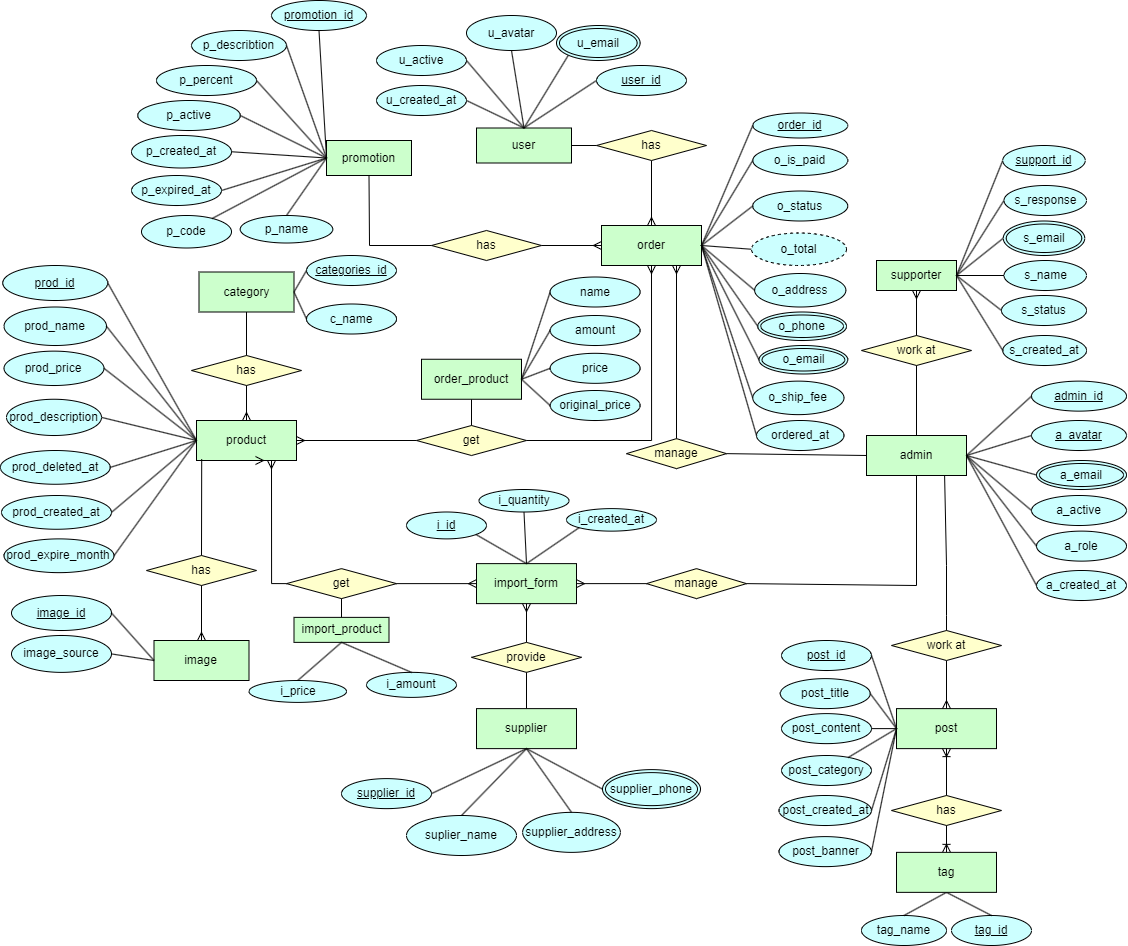
\includegraphics[width=1.1\textwidth]{ERD.png}
  \caption{ERD Diagram}
  \label{fig:erd}
\end{figure}

%giải thích các thực thể và mối quan hệ giữa các thực thể


\subsection{Physical Database Diagram}
\begin{figure}[H]
  \centering
  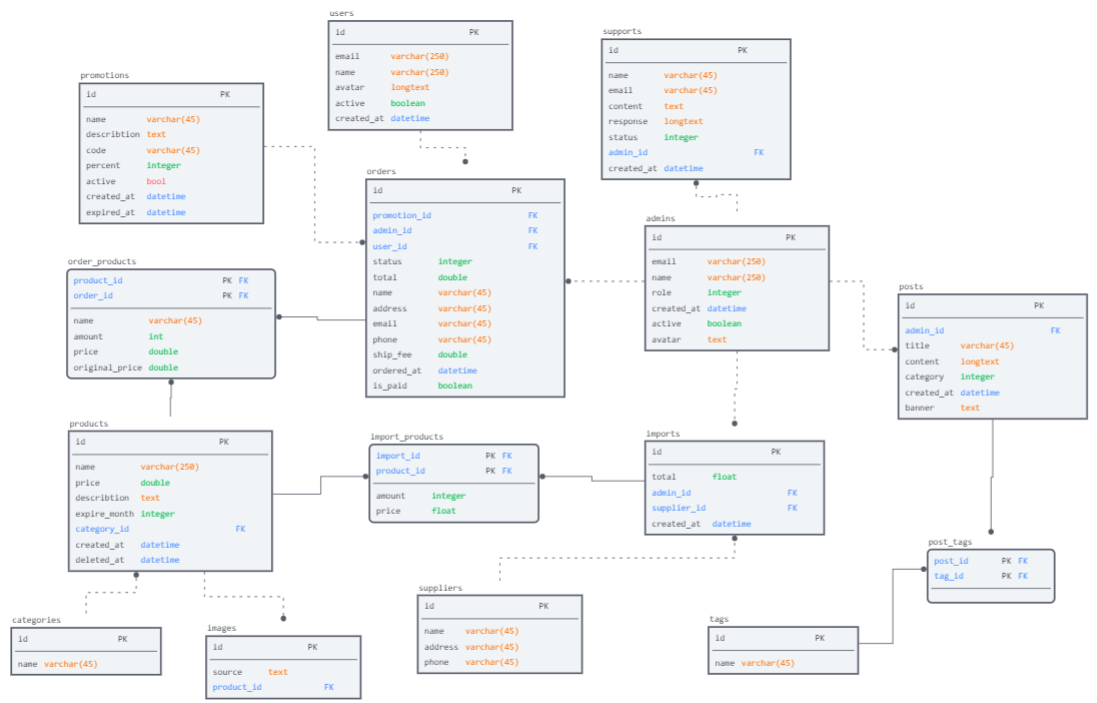
\includegraphics[width=1.1\textwidth]{physical.png}
  \caption{Physical Database Diagram}
  \label{fig:physicaldatabase}
\end{figure}


\section{Data Flow Diagram (DFD)}
\textbf{* Overview:}\\
The DFD diagram of a coffee shop website illustrates the activities, processes, and data flows within the system. It includes main components such as Customer, Admin, Employees, and related data tables. \\
Customers can perform operations such as viewing/searching for products, placing orders, and making payments, while Admin and Employees can perform management activities like product management, order processing, and payment processing. Data related to products, orders, and payments are stored in data tables that are managed and updated by Admins and Employees. The DFD diagram also depicts order processing, including order confirmation, product inspection, and invoicing. Additionally, customers can read articles and blogs about coffee, which are managed by Marketing Employees and then displayed on the website for the customers. \\ Overall, the DFD diagram provides an overview of the activities and data flows within the website's system, from logging in and viewing products to ordering and paying, performed by Customers, Admins, and Employees.
\subsection{DFD Context}

\begin{figure}[H]
  \centering
  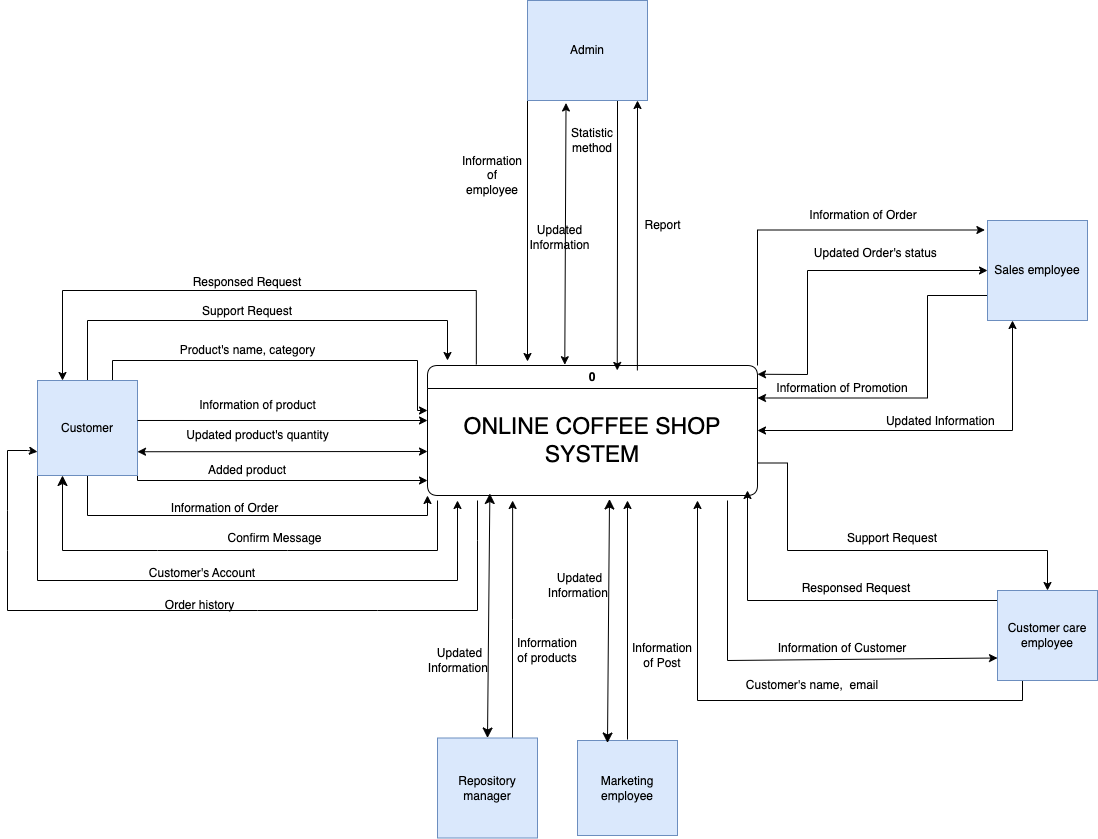
\includegraphics[width=1.1\textwidth]{DFDContext.png}
  \caption{DFD Context}
  \label{fig:dfdcontext}
\end{figure}

\subsection{DFD Level 0}
\textbf{* Overview:} \\
DFD Level 0 has: \\ 
+ 12 main processes: View statistics, Manage employee, Manage customer, Manage product and repository, Manage post, Manage promotion, Manage order, Send a support request, Search/View product, Manage Cart, Order, and View order history. \\
+ 6 external entities: Admin, Sales employee, Customer care employee, Marketing employee, Repository manager, and Customer.
\begin{figure}[H]
  \centering
  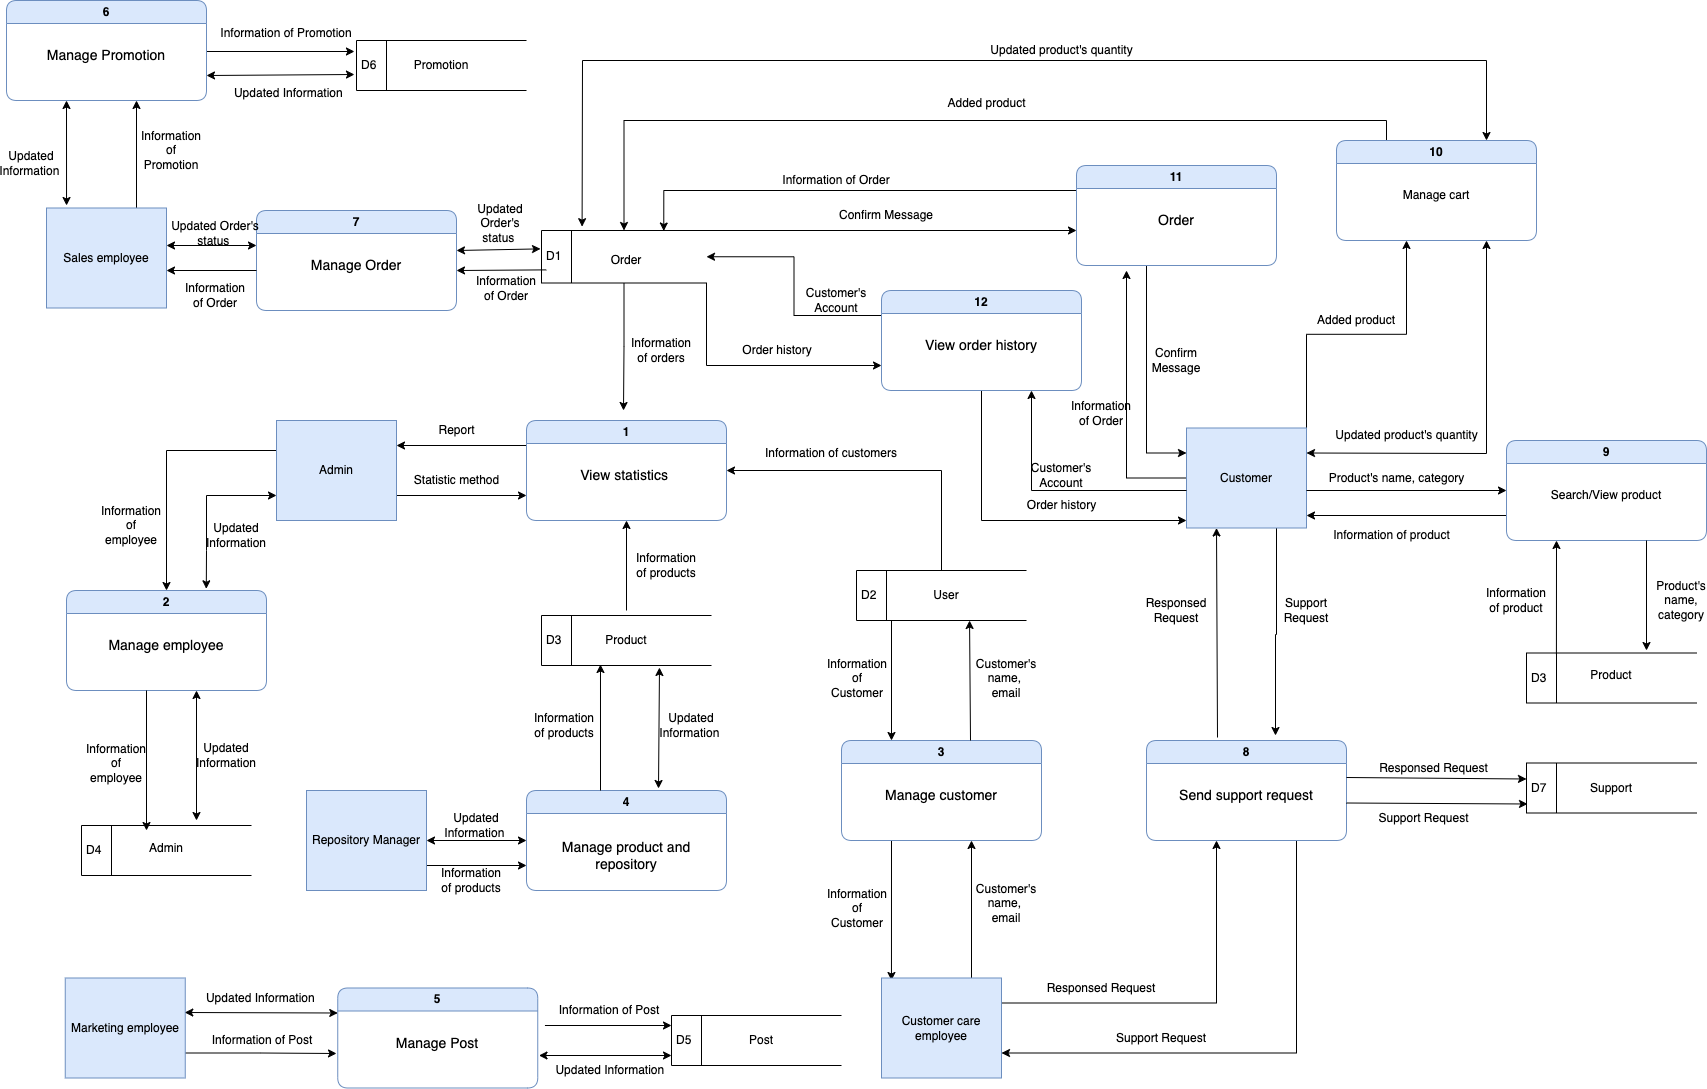
\includegraphics[width=1.1\textwidth]{DFDLevel0.png}
  \caption{DFD Level 0}
  \label{fig:dfdlevel0}
\end{figure}

* DFD Fragments
\begin{figure}[H]
  \centering
  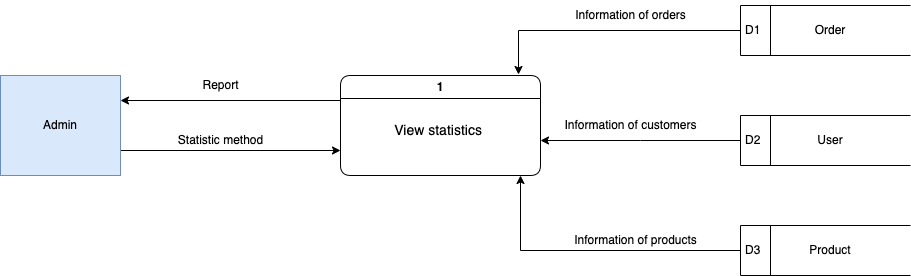
\includegraphics[width=1.1\textwidth]{DFD-UC02.png}
  \caption{DFD Fragment of UC02}
  \label{fig:dfd-uc02}
\end{figure}

\begin{figure}[H]
  \centering
  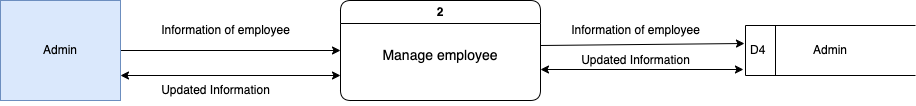
\includegraphics[width=1.1\textwidth]{DFD-UC03.png}
  \caption{DFD Fragment of UC03}
  \label{fig:dfd-uc03}
\end{figure}

\begin{figure}[H]
  \centering
  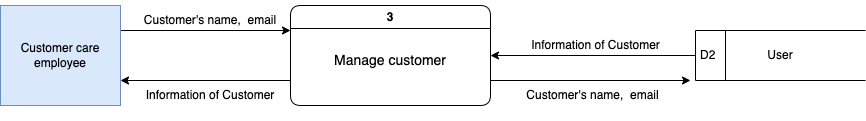
\includegraphics[width=1.1\textwidth]{DFD-UC04.png}
  \caption{DFD Fragment of UC04}
  \label{fig:dfd-uc04}
\end{figure}

\begin{figure}[H]
  \centering
  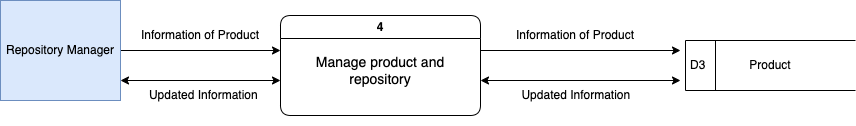
\includegraphics[width=1.1\textwidth]{DFD-UC05.png}
  \caption{DFD Fragment of UC05}
  \label{fig:dfd-uc05}
\end{figure}

\begin{figure}[H]
  \centering
  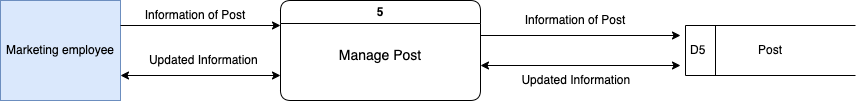
\includegraphics[width=1.1\textwidth]{DFD-UC06.png}
  \caption{DFD Fragment of UC06}
  \label{fig:dfd-uc06}
\end{figure}

\begin{figure}[H]
  \centering
  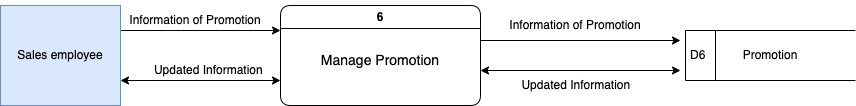
\includegraphics[width=1.1\textwidth]{DFD-UC07.png}
  \caption{DFD Fragment of UC07}
  \label{fig:dfd-uc07}
\end{figure}

\begin{figure}[H]
  \centering
  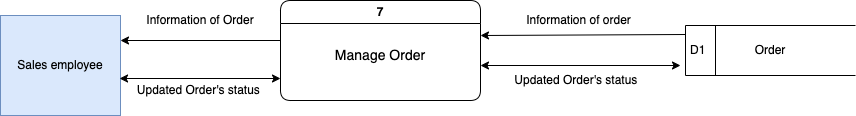
\includegraphics[width=1.1\textwidth]{DFD-UC08.png}
  \caption{DFD Fragment of UC08}
  \label{fig:dfd-uc08}
\end{figure}

\begin{figure}[H]
  \centering
  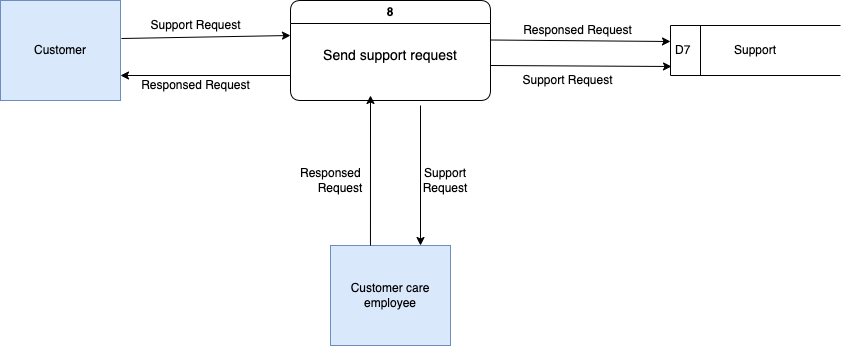
\includegraphics[width=1.1\textwidth]{DFD-UC09.png}
  \caption{DFD Fragment of UC09}
  \label{fig:dfd-uc09}
\end{figure}

\begin{figure}[H]
  \centering
  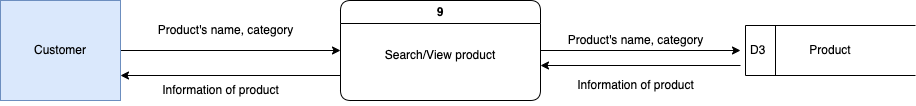
\includegraphics[width=1.1\textwidth]{DFD-UC10.png}
  \caption{DFD Fragment of UC010}
  \label{fig:dfd-uc010}
\end{figure}

\begin{figure}[H]
  \centering
  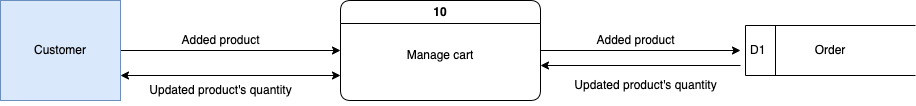
\includegraphics[width=1.1\textwidth]{DFD-UC11.png}
  \caption{DFD Fragment of UC011}
  \label{fig:dfd-uc011}
\end{figure}

\begin{figure}[H]
  \centering
  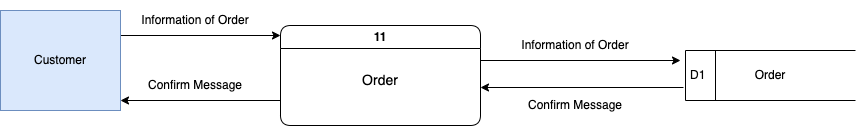
\includegraphics[width=1.1\textwidth]{DFD-UC12.png}
  \caption{DFD Fragment of UC012}
  \label{fig:dfd-uc012}
\end{figure}

\begin{figure}[H]
  \centering
  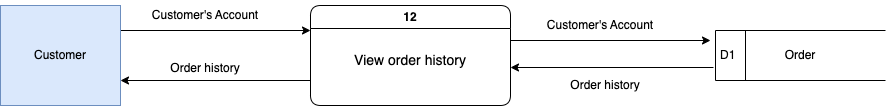
\includegraphics[width=1.1\textwidth]{DFD-UC13.png}
  \caption{DFD Fragment of UC013}
  \label{fig:dfd-uc013}
\end{figure}

